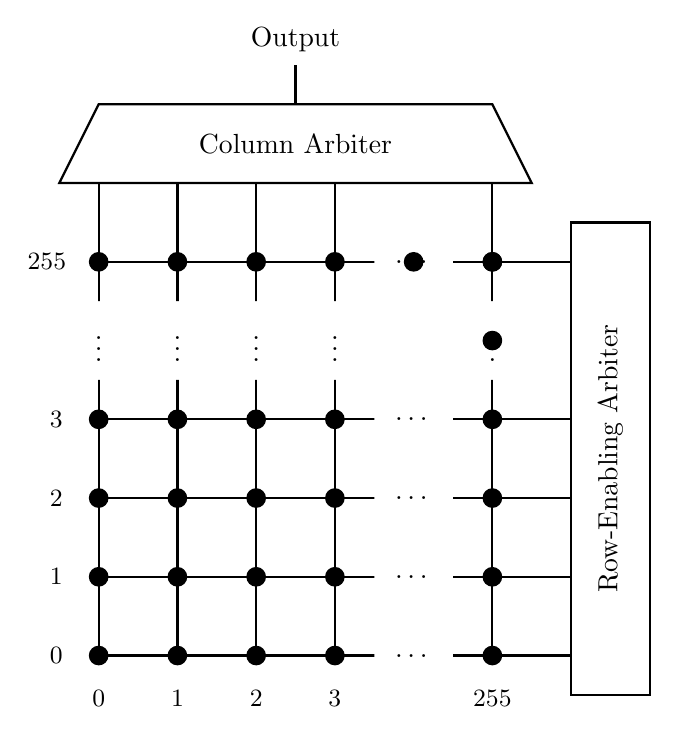
\begin{tikzpicture}[thick,minimum size=0.25cm,inner sep=0]
	\def\width{6}
	\def\height{6}
	\def\maxwidth{255}
	\def\maxheight{255}
	\pgfmathtruncatemacro{\widthh}{\width-1}
	\pgfmathtruncatemacro{\heightt}{\height-1}
	\pgfmathtruncatemacro{\widthhh}{\widthh-1}
	\pgfmathtruncatemacro{\heighttt}{\heightt-1}
	\pgfmathtruncatemacro{\widthhhh}{\widthhh-1}
	\pgfmathtruncatemacro{\heightttt}{\heighttt-1}
	
	% Nodes
	\foreach \x in {1,...,\widthhh}{
		\foreach \y in {1,...,\heighttt}{
			\node [fill,circle] at (\x,\y) (node X\x{}Y\y) {};
		}
	}
	
	% Outer nodes
	\foreach \x in {1,...,\width}{
		\ifthenelse{\x = \widthh}{}{
			\node [fill,circle] at (\x,\height) (node X\x{}Y\height) {};
		}
	}
	\foreach \y in {1,...,\height}{
		\ifthenelse{\y = \heightt}{}{
			\node [fill,circle] at (\width,\y) (node X\width{}Y\y) {};
		}
	}
	
	% Labels
	\foreach \x in {0,...,\widthhhh}{
		\node [anchor=north] at (1+\x,0.6) {\small{}\x};
	}
	\node [anchor=north] at (\height,0.6) {\small{}\maxwidth};
	\foreach \y in {0,...,\heightttt}{
		\node [anchor=east] at (0.6,1+\y) {\small{}\y};
	}
	\node [anchor=east] at (0.6,\height) {\small{}\maxheight};
	
	% Ellipsis
	\foreach \x in {1,...,\widthhh}{
		\node at (\x,\heightt) {\vdots};
	}
	\foreach \y in {1,...,\heighttt}{
		\node at (\widthh,\y)  {\ldots};
	}
	\node at (\widthh,\height)  {\ldots};
	\node at (\width,\heightt)  {\vdots};
	
	% Links
	\begin{scope}
		\clip (0.5,0.5) rectangle ++(\widthhh,\heighttt)
		      (0.5         ,1.5+\heighttt) rectangle ++(\widthhh,2)
		      (1.5+\widthhh,0.5          ) rectangle ++(2,\heighttt)
		      (1.5+\widthhh,1.5+\heighttt) rectangle ++(2,2)
		      ;
		
		\foreach \x in {1,...,\width}{
			\foreach \y in {1,...,\height}{
				\draw (\x,\y) -- ++( 1, 0);
				\draw (\x,\y) -- ++( 0, 1);
			}
		}
	\end{scope}
	
	% Arbiters
	\draw (1+\width,0.5)
	  --++(0, \height)
	  --++(1, 0)
	  --++(0, -\height)
	  --  cycle
	      ;
	\node at (1.5+\width,0.5+0.5*\height) [rotate=90] {Row-Enabling Arbiter};
	\draw (0.5,1+\height)
	  --++(\width, 0)
	  --++(-0.5, 1)
	  --++(-\widthh, 0)
	  --  cycle
	      ;
	\node at (0.5+0.5*\width,1.5+\height) {Column Arbiter};
	
	% Output
	\draw (0.5+0.5*\width,2+\height)
	   -- ++(0, 0.5)
	 node [anchor=south,yshift=1ex]
	      {Output}
	      ;
\end{tikzpicture}
